\section{Apriori$<$ Sets\-Type, Measure, Cand\_\-Data\-Struct $>$ Class Template Reference}
\label{class_apriori}\index{Apriori@{Apriori}}
Functor finding the theory and/or the negative border and/or the positive border using the algorithm {\bf Apriori}{\rm (p.\,\pageref{class_apriori})}.  


{\tt \#include $<$Apriori.hxx$>$}

Inheritance diagram for Apriori$<$ Sets\-Type, Measure, Cand\_\-Data\-Struct $>$::\begin{figure}[H]
\begin{center}
\leavevmode
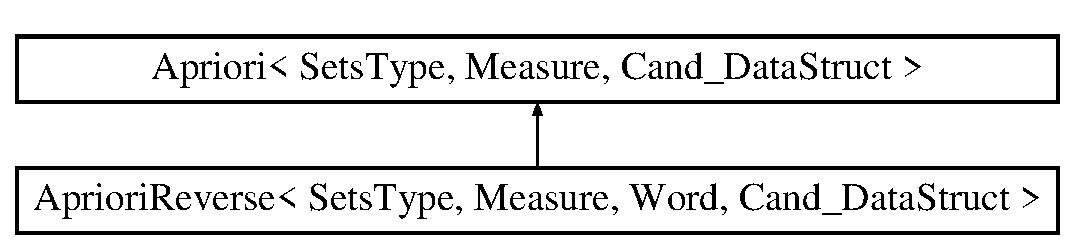
\includegraphics[height=2cm]{class_apriori}
\end{center}
\end{figure}
\subsection*{Public Member Functions}
\begin{CompactItemize}
\item 
template$<$class Init\-Functor, class Predicate, class Output\-Theory, class Output\-Bd\-P, class Output\-Bd\-N, class f, class Stop\-Iteration, class f2$>$ void {\bf execute\-Algo} (Init\-Functor \&init, {\bf Predicate} $\ast$pred, Output\-Theory $\ast$theory, Output\-Bd\-P $\ast$bd\-P, Output\-Bd\-N $\ast$bd\-N, f \&word\-To\-Set, Stop\-Iteration $\ast$stop\-Ite, f2 \&word\-To\-Set\-Save, deque$<$ Sets\-Type $>$ $\ast$list\-Interes\-Items=0)
\begin{CompactList}\small\item\em Function that execute the algorithm operator that executes the algorithm. \item\end{CompactList}\item 
{\bf Apriori} ()\label{class_apriori_8287a89c0b7f56a814f945e75ca29f0d}

\begin{CompactList}\small\item\em Constructor. \item\end{CompactList}\item 
template$<$class Init\-Functor, class Predicate, class Output\-Theory, class Output\-Bd\-P, class Output\-Bd\-N, class f$>$ void {\bf operator()} (Init\-Functor \&init, {\bf Predicate} \&pred, Output\-Theory $\ast$theory, Output\-Bd\-P $\ast$bd\-P, Output\-Bd\-N $\ast$bd\-N, f \&word\-To\-Set)
\begin{CompactList}\small\item\em Functor operator that executes the algorithm. \item\end{CompactList}\item 
template$<$class Init\-Functor, class Predicate, class Output\-Theory, class Output\-Bd\-P, class Output\-Bd\-N$>$ void {\bf operator()} (Init\-Functor \&init, {\bf Predicate} \&pred, Output\-Theory $\ast$theory, Output\-Bd\-P $\ast$bd\-P, Output\-Bd\-N $\ast$bd\-N)
\begin{CompactList}\small\item\em Functor operator that executes the algorithm. \item\end{CompactList}\item 
template$<$class Init\-Functor, class Predicate, class Output\-Theory, class Output\-Bd\-P, class Output\-Bd\-N, class f, class Stop\-Iteration$>$ void {\bf operator()} (Init\-Functor \&init, {\bf Predicate} \&pred, Output\-Theory $\ast$theory, Output\-Bd\-P $\ast$bd\-P, Output\-Bd\-N $\ast$bd\-N, Stop\-Iteration $\ast$stop\-Ite, f \&word\-To\-Set)
\begin{CompactList}\small\item\em Functor operator that executes the algorithm and stop his execution when the functor passed in parameter return false. \item\end{CompactList}\item 
template$<$class Init\-Functor, class Predicate, class Output\-Theory, class Output\-Bd\-P, class Output\-Bd\-N, class Stop\-Iteration$>$ void {\bf operator()} (Init\-Functor \&init, {\bf Predicate} \&pred, Output\-Theory $\ast$theory, Output\-Bd\-P $\ast$bd\-P, Output\-Bd\-N $\ast$bd\-N, Stop\-Iteration $\ast$stop\-Ite)
\begin{CompactList}\small\item\em Functor operator that executes the algorithm and stop his execution when the functor passed in parameter return false. \item\end{CompactList}\end{CompactItemize}
\subsection*{Public Attributes}
\begin{CompactItemize}
\item 
bool {\bf verbose}\label{class_apriori_de33c80face437efdf4b032849811d07}

\begin{CompactList}\small\item\em {\bf Boolean}{\rm (p.\,\pageref{class_boolean})} to print to screen some informations during the execution (default false). \item\end{CompactList}\item 
bool {\bf save\-Set}\label{class_apriori_7fd142ed119cef31fdcb325709425ab6}

\begin{CompactList}\small\item\em {\bf Boolean}{\rm (p.\,\pageref{class_boolean})} to save the set representation of the solution. \item\end{CompactList}\end{CompactItemize}
\subsection*{Protected Member Functions}
\begin{CompactItemize}
\item 
template$<$class Iterator$>$ bool {\bf test\-Subset} (Iterator \&it\-Pref, Iterator \&it\-Last, vector$<$ Sets\-Type $>$ \&buffer)
\begin{CompactList}\small\item\em Test if a set generated using the elements pointed by it\-Pref and it\-Last is a candidate. \item\end{CompactList}\item 
template$<$class Iterator$>$ void {\bf erase\-Subset} (Cand\_\-Data\-Struct \&cand, Iterator \&position, vector$<$ Sets\-Type $>$ \&buffer)
\begin{CompactList}\small\item\em Erase all the k-1 subsets of the set of size k coresponding to the iterator in parameter. \item\end{CompactList}\item 
void {\bf filter} (Cand\_\-Data\-Struct \&cand)
\begin{CompactList}\small\item\em Filter the elements of the positive border from the theory. \item\end{CompactList}\item 
int {\bf candidates\-Generation} (Cand\_\-Data\-Struct \&cand, int \&level)
\begin{CompactList}\small\item\em Candidate generation phase of {\bf Apriori}{\rm (p.\,\pageref{class_apriori})}. \item\end{CompactList}\item 
template$<$class Predicate, class Output\-Theory, class Output\-Bd\-N, class f, class f2$>$ int {\bf prune} (Cand\_\-Data\-Struct \&cand, {\bf Predicate} $\ast$pred, Output\-Theory $\ast$theory, Output\-Bd\-N $\ast$bd\-N, f \&word\-To\-Set, f2 \&word\-To\-Set\-Save, deque$<$ Sets\-Type $>$ $\ast$list\-Interes\-Items=0)
\begin{CompactList}\small\item\em Pruning generation phase of {\bf Apriori}{\rm (p.\,\pageref{class_apriori})}. \item\end{CompactList}\end{CompactItemize}
\subsection*{Protected Attributes}
\begin{CompactItemize}
\item 
Cand\_\-Data\-Struct {\bf candidates}\label{class_apriori_7a7457c2cb4aacb56a88c1f70bfa5b88}

\begin{CompactList}\small\item\em The candidates generated. \item\end{CompactList}\end{CompactItemize}
\subsection*{Classes}
\begin{CompactItemize}
\item 
class {\bf init\-Candidates}
\begin{CompactList}\small\item\em Initialize the set of candidates with the basic words of the language. \item\end{CompactList}\end{CompactItemize}


\subsection{Detailed Description}
\subsubsection*{template$<$class Sets\-Type = int, class Measure = Boolean, class Cand\_\-Data\-Struct = PTree$<$Sets\-Type,Measure$>$$>$ class Apriori$<$ Sets\-Type, Measure, Cand\_\-Data\-Struct $>$}

Functor finding the theory and/or the negative border and/or the positive border using the algorithm {\bf Apriori}{\rm (p.\,\pageref{class_apriori})}. 

This class enables the execution of the classic {\bf Apriori}{\rm (p.\,\pageref{class_apriori})} algorithm. Moreover this class enables to stop the execution of {\bf Apriori}{\rm (p.\,\pageref{class_apriori})} at an iteration wrt to a user defined functor. The template parameter Sets\-Type represents the type of the sets representing the elements of the language. The template parameter Measure is the type of the value eventually associated with the word of the language. The template parameter Cand\_\-Data\-Struct is the data structure type used to store the candidates generated by the algorithms. 



\subsection{Member Function Documentation}
\index{Apriori@{Apriori}!candidatesGeneration@{candidatesGeneration}}
\index{candidatesGeneration@{candidatesGeneration}!Apriori@{Apriori}}
\subsubsection{\setlength{\rightskip}{0pt plus 5cm}template$<$class Sets\-Type, class Measure, class Cand\_\-Data\-Struct$>$ int {\bf Apriori}$<$ Sets\-Type, Measure, Cand\_\-Data\-Struct $>$::candidates\-Generation (Cand\_\-Data\-Struct \& {\em cand}, int \& {\em level})\hspace{0.3cm}{\tt  [protected]}}\label{class_apriori_f7d6a2dbd1c203246f36081ca1f0e325}


Candidate generation phase of {\bf Apriori}{\rm (p.\,\pageref{class_apriori})}. 

\begin{Desc}
\item[Parameters:]
\begin{description}
\item[{\em cand}]set of candidates. \item[{\em level}]current size of the candidates \end{description}
\end{Desc}
\begin{Desc}
\item[Returns:]the number of sets generated. \end{Desc}
\index{Apriori@{Apriori}!eraseSubset@{eraseSubset}}
\index{eraseSubset@{eraseSubset}!Apriori@{Apriori}}
\subsubsection{\setlength{\rightskip}{0pt plus 5cm}template$<$class Sets\-Type, class Measure, class Cand\_\-Data\-Struct$>$ template$<$class Iterator$>$ void {\bf Apriori}$<$ Sets\-Type, Measure, Cand\_\-Data\-Struct $>$::erase\-Subset (Cand\_\-Data\-Struct \& {\em cand}, Iterator \& {\em position}, vector$<$ Sets\-Type $>$ \& {\em buffer})\hspace{0.3cm}{\tt  [protected]}}\label{class_apriori_ea2d007414bb3735d61a1b27a2b14667}


Erase all the k-1 subsets of the set of size k coresponding to the iterator in parameter. 

\begin{Desc}
\item[Parameters:]
\begin{description}
\item[{\em cand}]contains the theory. \item[{\em position}]iterator on the set. \item[{\em buffer}]container of size k used to test subset. \end{description}
\end{Desc}
\index{Apriori@{Apriori}!executeAlgo@{executeAlgo}}
\index{executeAlgo@{executeAlgo}!Apriori@{Apriori}}
\subsubsection{\setlength{\rightskip}{0pt plus 5cm}template$<$class Sets\-Type, class Measure, class Cand\_\-Data\-Struct$>$ template$<$class Init\-Functor, class Predicate, class Output\-Theory, class Output\-Bd\-P, class Output\-Bd\-N, class f, class Stop\-Iteration, class f2$>$ void {\bf Apriori}$<$ Sets\-Type, Measure, Cand\_\-Data\-Struct $>$::execute\-Algo (Init\-Functor \& {\em init}, {\bf Predicate} $\ast$ {\em pred}, Output\-Theory $\ast$ {\em theory}, Output\-Bd\-P $\ast$ {\em bd\-P}, Output\-Bd\-N $\ast$ {\em bd\-N}, f \& {\em word\-To\-Set}, Stop\-Iteration $\ast$ {\em stop\-Ite}, f2 \& {\em word\-To\-Set\-Save}, deque$<$ Sets\-Type $>$ $\ast$ {\em list\-Interes\-Items} = {\tt 0})}\label{class_apriori_cef957e8ca48064546d3aed66c1927c7}


Function that execute the algorithm operator that executes the algorithm. 

\begin{Desc}
\item[Parameters:]
\begin{description}
\item[{\em init}]functor initializing the interesting items wrt predicate. \item[{\em pred}]the predicate \item[{\em theory}]output the theory in the given objet (must have a push\_\-back( container, measure ) method). \item[{\em bd\-P}]output the positive border in the given objet (must have a push\_\-back( container, measure ) method). \item[{\em bd\-N}]output the negative border in the given objet (must have a push\_\-back( container, measure ) method). \item[{\em set\-To\-Word}]transform words of the language studied in sets. \item[{\em stop\-Ite}]functor stop that stop the execution of apriori before the end. \item[{\em set\-To\-Word\-Save}]transform for output the sets find by the algorithm in words of the language. \item[{\em list\-Interest\-Items}]list of all the interesting items (set representation). \end{description}
\end{Desc}
\index{Apriori@{Apriori}!filter@{filter}}
\index{filter@{filter}!Apriori@{Apriori}}
\subsubsection{\setlength{\rightskip}{0pt plus 5cm}template$<$class Sets\-Type, class Measure, class Cand\_\-Data\-Struct$>$ void {\bf Apriori}$<$ Sets\-Type, Measure, Cand\_\-Data\-Struct $>$::filter (Cand\_\-Data\-Struct \& {\em cand})\hspace{0.3cm}{\tt  [protected]}}\label{class_apriori_44e415598f2de8a80b341c53dce01b12}


Filter the elements of the positive border from the theory. 

\begin{Desc}
\item[Parameters:]
\begin{description}
\item[{\em cand}]contains the theory. \end{description}
\end{Desc}
\index{Apriori@{Apriori}!operator()@{operator()}}
\index{operator()@{operator()}!Apriori@{Apriori}}
\subsubsection{\setlength{\rightskip}{0pt plus 5cm}template$<$class Sets\-Type = int, class Measure = Boolean, class Cand\_\-Data\-Struct = PTree$<$Sets\-Type,Measure$>$$>$ template$<$class Init\-Functor, class Predicate, class Output\-Theory, class Output\-Bd\-P, class Output\-Bd\-N, class Stop\-Iteration$>$ void {\bf Apriori}$<$ Sets\-Type, Measure, Cand\_\-Data\-Struct $>$::operator() (Init\-Functor \& {\em init}, {\bf Predicate} \& {\em pred}, Output\-Theory $\ast$ {\em theory}, Output\-Bd\-P $\ast$ {\em bd\-P}, Output\-Bd\-N $\ast$ {\em bd\-N}, Stop\-Iteration $\ast$ {\em stop\-Ite})\hspace{0.3cm}{\tt  [inline]}}\label{class_apriori_117edc08779546395973171927fb8a77}


Functor operator that executes the algorithm and stop his execution when the functor passed in parameter return false. 

\begin{Desc}
\item[Parameters:]
\begin{description}
\item[{\em init}]functor initializing the interesting items wrt predicate. \item[{\em pred}]the predicate \item[{\em theory}]output the theory in the given objet (must have a push\_\-back( container, measure ) method). \item[{\em bd\-P}]output the positive border in the given objet (must have a push\_\-back( container, measure ) method). \item[{\em bd\-N}]output the negative border in the given objet (must have a push\_\-back( container, measure ) method). \item[{\em stop\-Ite}]functor stop that stop the execution of apriori before the end. \item[{\em word\-To\-Set}]transform words of the language studied in sets. \end{description}
\end{Desc}


Reimplemented in {\bf Apriori\-Reverse$<$ Sets\-Type, Measure, Word, Cand\_\-Data\-Struct $>$} {\rm (p.\,\pageref{class_apriori_reverse_a8018f226acaaa0047cf1386ed189e08})}.\index{Apriori@{Apriori}!operator()@{operator()}}
\index{operator()@{operator()}!Apriori@{Apriori}}
\subsubsection{\setlength{\rightskip}{0pt plus 5cm}template$<$class Sets\-Type = int, class Measure = Boolean, class Cand\_\-Data\-Struct = PTree$<$Sets\-Type,Measure$>$$>$ template$<$class Init\-Functor, class Predicate, class Output\-Theory, class Output\-Bd\-P, class Output\-Bd\-N, class f, class Stop\-Iteration$>$ void {\bf Apriori}$<$ Sets\-Type, Measure, Cand\_\-Data\-Struct $>$::operator() (Init\-Functor \& {\em init}, {\bf Predicate} \& {\em pred}, Output\-Theory $\ast$ {\em theory}, Output\-Bd\-P $\ast$ {\em bd\-P}, Output\-Bd\-N $\ast$ {\em bd\-N}, Stop\-Iteration $\ast$ {\em stop\-Ite}, f \& {\em word\-To\-Set})\hspace{0.3cm}{\tt  [inline]}}\label{class_apriori_4ccc3fe5ae7ecaa9efffcdc41d1888ed}


Functor operator that executes the algorithm and stop his execution when the functor passed in parameter return false. 

\begin{Desc}
\item[Parameters:]
\begin{description}
\item[{\em init}]functor initializing the interesting items wrt predicate. \item[{\em pred}]the predicate \item[{\em theory}]output the theory in the given objet (must have a push\_\-back( container, measure ) method). \item[{\em bd\-P}]output the positive border in the given objet (must have a push\_\-back( container, measure ) method). \item[{\em bd\-N}]output the negative border in the given objet (must have a push\_\-back( container, measure ) method). \item[{\em stop\-Ite}]functor stop that stop the execution of apriori before the end. \item[{\em word\-To\-Set}]transform words of the language studied in sets. \end{description}
\end{Desc}


Reimplemented in {\bf Apriori\-Reverse$<$ Sets\-Type, Measure, Word, Cand\_\-Data\-Struct $>$} {\rm (p.\,\pageref{class_apriori_reverse_d898f211e89442230c64651031388e3d})}.\index{Apriori@{Apriori}!operator()@{operator()}}
\index{operator()@{operator()}!Apriori@{Apriori}}
\subsubsection{\setlength{\rightskip}{0pt plus 5cm}template$<$class Sets\-Type = int, class Measure = Boolean, class Cand\_\-Data\-Struct = PTree$<$Sets\-Type,Measure$>$$>$ template$<$class Init\-Functor, class Predicate, class Output\-Theory, class Output\-Bd\-P, class Output\-Bd\-N$>$ void {\bf Apriori}$<$ Sets\-Type, Measure, Cand\_\-Data\-Struct $>$::operator() (Init\-Functor \& {\em init}, {\bf Predicate} \& {\em pred}, Output\-Theory $\ast$ {\em theory}, Output\-Bd\-P $\ast$ {\em bd\-P}, Output\-Bd\-N $\ast$ {\em bd\-N})\hspace{0.3cm}{\tt  [inline]}}\label{class_apriori_f0a2087314d1753cc3dd397c4a3f3dda}


Functor operator that executes the algorithm. 

\begin{Desc}
\item[Parameters:]
\begin{description}
\item[{\em init}]functor initializing the interesting items wrt predicate. \item[{\em pred}]the predicate \item[{\em theory}]output the theory in the given objet (must have a push\_\-back( container, measure ) method). \item[{\em bd\-P}]output the positive border in the given objet (must have a push\_\-back( container, measure ) method). \item[{\em bd\-N}]output the negative border in the given objet (must have a push\_\-back( container, measure ) method). \end{description}
\end{Desc}


Reimplemented in {\bf Apriori\-Reverse$<$ Sets\-Type, Measure, Word, Cand\_\-Data\-Struct $>$} {\rm (p.\,\pageref{class_apriori_reverse_5266cde8d5a9455c9f9281e435754ca9})}.\index{Apriori@{Apriori}!operator()@{operator()}}
\index{operator()@{operator()}!Apriori@{Apriori}}
\subsubsection{\setlength{\rightskip}{0pt plus 5cm}template$<$class Sets\-Type = int, class Measure = Boolean, class Cand\_\-Data\-Struct = PTree$<$Sets\-Type,Measure$>$$>$ template$<$class Init\-Functor, class Predicate, class Output\-Theory, class Output\-Bd\-P, class Output\-Bd\-N, class f$>$ void {\bf Apriori}$<$ Sets\-Type, Measure, Cand\_\-Data\-Struct $>$::operator() (Init\-Functor \& {\em init}, {\bf Predicate} \& {\em pred}, Output\-Theory $\ast$ {\em theory}, Output\-Bd\-P $\ast$ {\em bd\-P}, Output\-Bd\-N $\ast$ {\em bd\-N}, f \& {\em word\-To\-Set})\hspace{0.3cm}{\tt  [inline]}}\label{class_apriori_36d7a2cdad2a8c459f2b44e3ab460591}


Functor operator that executes the algorithm. 

\begin{Desc}
\item[Parameters:]
\begin{description}
\item[{\em init}]functor initializing the interesting items wrt predicate. \item[{\em pred}]the predicate \item[{\em theory}]output the theory in the given objet (must have a push\_\-back( container, measure ) method). \item[{\em bd\-P}]output the positive border in the given objet (must have a push\_\-back( container, measure ) method). \item[{\em bd\-N}]output the negative border in the given objet (must have a push\_\-back( container, measure ) method). \item[{\em word\-To\-Set}]transform words of the language studied in sets. \end{description}
\end{Desc}


Reimplemented in {\bf Apriori\-Reverse$<$ Sets\-Type, Measure, Word, Cand\_\-Data\-Struct $>$} {\rm (p.\,\pageref{class_apriori_reverse_f82618122967f0c6da9c4de5ea60a367})}.\index{Apriori@{Apriori}!prune@{prune}}
\index{prune@{prune}!Apriori@{Apriori}}
\subsubsection{\setlength{\rightskip}{0pt plus 5cm}template$<$class Sets\-Type, class Measure, class Cand\_\-Data\-Struct$>$ template$<$class Predicate, class Output\-Theory, class Output\-Bd\-N, class f, class f2$>$ int {\bf Apriori}$<$ Sets\-Type, Measure, Cand\_\-Data\-Struct $>$::prune (Cand\_\-Data\-Struct \& {\em cand}, {\bf Predicate} $\ast$ {\em pred}, Output\-Theory $\ast$ {\em theory}, Output\-Bd\-N $\ast$ {\em bd\-N}, f \& {\em word\-To\-Set}, f2 \& {\em word\-To\-Set\-Save}, deque$<$ Sets\-Type $>$ $\ast$ {\em list\-Interes\-Items} = {\tt 0})\hspace{0.3cm}{\tt  [protected]}}\label{class_apriori_a9bea497daba465a98b5ff9e933c2b27}


Pruning generation phase of {\bf Apriori}{\rm (p.\,\pageref{class_apriori})}. 

\begin{Desc}
\item[Parameters:]
\begin{description}
\item[{\em cand}]set of candidates. \item[{\em pred}]the predicate. \item[{\em bd\-N}]output the negative border in the given objet (must have a push\_\-back( container, measure ) method). \item[{\em theory}]output the theory in the given objet (must have a push\_\-back( container, measure ) method). \item[{\em set\-To\-Word\-Save}]transform for output the sets find by the algorithm in words of the language. \item[{\em list\-Interest\-Items}]list of all the interesting items (set representation). \end{description}
\end{Desc}
\begin{Desc}
\item[Returns:]the number of candidates pruned. \end{Desc}
\index{Apriori@{Apriori}!testSubset@{testSubset}}
\index{testSubset@{testSubset}!Apriori@{Apriori}}
\subsubsection{\setlength{\rightskip}{0pt plus 5cm}template$<$class Sets\-Type, class Measure, class Cand\_\-Data\-Struct$>$ template$<$class Iterator$>$ bool {\bf Apriori}$<$ Sets\-Type, Measure, Cand\_\-Data\-Struct $>$::test\-Subset (Iterator \& {\em it\-Pref}, Iterator \& {\em it\-Last}, vector$<$ Sets\-Type $>$ \& {\em buffer})\hspace{0.3cm}{\tt  [protected]}}\label{class_apriori_c86b934cfaf6e553ff92e8930eadf4b7}


Test if a set generated using the elements pointed by it\-Pref and it\-Last is a candidate. 

\begin{Desc}
\item[Parameters:]
\begin{description}
\item[{\em it\-Pref}]iterator on the prefix of the set to test. \item[{\em it\-Last}]iterator on the elemnt to add to form the candidate set. \item[{\em buffer}]container of size k used to test subset. \end{description}
\end{Desc}
\begin{Desc}
\item[Returns:]true if all the subsets of size k are already in the candidate. \end{Desc}


The documentation for this class was generated from the following file:\begin{CompactItemize}
\item 
F:/i\-Zi/algorithms/Apriori.hxx\end{CompactItemize}
